\documentclass[a4paper, 10pt]{article}
\usepackage[utf8x]{inputenc}
\usepackage[norsk]{babel}
\usepackage{natbib}
\usepackage{graphicx}
\usepackage[T1]{fontenc}
\usepackage{algpseudocode}


\title{Datamaskiner Grunnkurs}
\author{Kristoffer Dalby}
\date{}


\begin{document}

\maketitle

\thispagestyle{empty}
\newpage
\pagenumbering{arabic}
\setcounter{page}{1}

\section{Forkortelser}
 \begin{tabular}{|l|l|}
    \hline
    Forkortelse & Betydning                        \\ \hline
    PC          & Program Counter                  \\ \hline
    MPC         & Micro Program Counter            \\ \hline
    MBR         & Memory Buffer Register           \\ \hline
    IR          & Instruction Register             \\ \hline
    MAR         & Memory Address Register          \\ \hline
    MDR         & Memory Data Register             \\ \hline
    LV          & Local Variable                   \\ \hline
    SP          & Stack Pointer                    \\ \hline
    CPP         & Constant Pool Pointer            \\ \hline
    TOS         & Top Of Stack                     \\ \hline
    OPC         & OpCode                           \\ \hline
    H           & Holding Register                 \\ \hline
    ALU         & Arithmetic Logic Unit            \\ \hline
    RAW         & Read-After-Write                 \\ \hline
    WAW         & Write-After-Write                \\ \hline
    WAR         & Write-After-Read                 \\ \hline
    SRAM        & Static RAM                       \\ \hline
    SDRAM       & Synchronous Dynamic RAM          \\ \hline
    DRAM        & Dynamic RAM                      \\ \hline
    CMP         & Chip-level MultiProsessor        \\ \hline
    ILP         & Instruction-Level Parallelism    \\ \hline
    RISC        & Reduced Instruction Set Computer \\ \hline
    CISC        & Complex Instruction Set Computer \\ \hline
    MIR         & MicroInstruction Register        \\ \hline
    ~           & ~                                \\ \hline
    ~           & ~                                \\ \hline
    ~           & ~                                \\ \hline
    ~           & ~                                \\ \hline
    ~           & ~                                \\ \hline
    \end{tabular}
\newpage    
   
\section{Registre}
\subsection{PC}
Program counter peker på den instruksjonen i programmet som blir jobbet med.

\subsection{MPC}
Micro Program Counter peker på microinstruksjonen i 'control store'.  Den peker på den første micro instruksjonen i den aktive instruksjonen. MPC holder orden på hva den neste micro instruksjonen er.

\subsection{MBR}
Memory Buffer Register er et bufferregister mellom minne og prosessor.

\subsection{IR}
Instruction Register er der kontrollenheten lagrer instruksjonen som blir gjennomført nå. Den ligger her mens instruksjonen blir dekodet, startet og gjennomført.

\subsection{MAR}
Memory Address Register inneholder adresse til neste minnelokasjon der vi finner neste instruksjon.

\subsection{MDR}
Memory Data Register inneholder data som skal bli lagret i hovedminne/RAM, eller data som har blitt hentet fra minne. Det fungerer som en buffer så data er klar for prosessoren.

\subsection{LV}
Local Variable inneholder pekerverdi, den peker til det nederste elementet i stakken.

\subsection{SP}
Stack Pointer inneholder pekerverdi mot det øverste elementet i stakken.

\subsection{CPP}
Constant Pool Pointer inneholder pekerverdi. Kontanter fra Java-program, leses inn ved oppstart, endres ikke.

\subsection{TOS}
Top Of Stack skal alltid inneholde elementet på toppen av stakken

\subsection{OPC}
OpCode register kan fritt brukes.

\subsection{H}
Holding Register inneholder verdien som skal inn i A-inngangen til ALU.

\section{ALU-flagg}
\begin{tabular}{|l|l|}
    \hline
    Flagg & Årsak                                        \\ \hline
    N     & Når svar er negativt                         \\ \hline
    Z     & Når svaret er 0                              \\ \hline
    C     & Carry, når vi legger sammen uten fortegnsbit \\ \hline
    V     & Overflow                                     \\ \hline
\end{tabular}

\section{Von Neumann}
Data og instruksjoner er lagret i samme minne og beregninger skjer sekvensielt. Von Neumann-arkitektur gjør det mulig å skrive program som kan endre sin egen programkode.

\begin{figure}[hbt]
    \begin{center}
        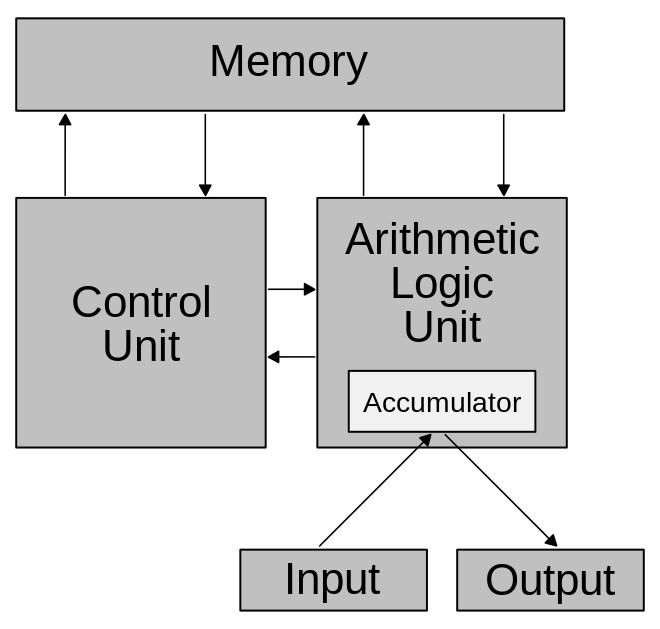
\includegraphics[width=6cm] {img/vonneumann.png}
        \caption{Et eksempel på Von Neumann}
    \end{center}
\end{figure}

\begin{itemize}
	\item ALU - Aritmetisk og logisk enhet som utfører beregningene.
	\item Control Unit - Kontrollenhet som dekoder instruksjoner og gjennomfører dem. \\ Kontrollenheten kan enten være hard-wired eller inneholde kode styrt av en mikrokontroller.
	\item Memory - Primærminnet (RAM) inneholder data og instruksjoner.
	\item I/O - Enheter for inn- og utdata.
	
\end{itemize}

Moderne datamaskiner har ALU og kontrollenhet på prosessor (CPU), benytter seg av registre, hurtigbuffere, busser og millioner av transistorer, men konseptet er veldig likt. Overføring av data mellom minne og CPU blir i dag sett på som et av de største problemene med Von Neumann-arkitektur.



\section{MicroInstruction Register}
\begin{itemize}
	\item Addr - Peker på neste mikroinstruksjon i instruksjonen.
	\item J - Jam sier ifra om ALU har flagget neste mikroinstruksjon eller om det kommer hopp (betinget hopp).
	\item Jam + Addr - Bestemmer neste mikroinstruksjon
	\item ALU - bestemmer hvilken funksjon ALU skal gjennomføre.
	\item C - Inneholder adressen til C-bussen, som blir det samme som adressen til registeret det skal skrives til. 
	\item Mem - Sier ifra om det skal gjøres noe med minne.
	\item B - inneholder adressen til B-bussen, som blir det samme som adressen til registeret det skal leses fra.
\end{itemize}

\section{Superskalar CPU}
En superskalar prosessor implementerer en form for parallellitet som kalles instruksjonsnivåparallellitet. Dette betyr at den kan utføre flere instruksjoner pr. klokkesyklus (dupliserer CPU-enheter). Duplisering av CPU komponenter. Billigere om man bare dupliserer noen.

\subsection{Klokkesyklus}
For å regne ut klokkesyklus med gitt forsinkelse tar man å deler 1 på 

\section{Lokalitet}
\subsection{Tid}
Om vi leste fra en minneadresse er det sannsynlig at vi snart vil lese fra den samme adressen igjen.

\subsection{Rom}
Om vi leste fra en minneadresse er det sannsynlig at vi snart vil lese fra naboadressen.

\section{Dataavhengighet}
\subsection{RAW}
Read-After-Write (sanne dataavhengigheter er når for eksempel instruksjon 1 skriver til et register og instruksjon 2 skal lese fra det samme registeret.

\subsection{WAW}
Write-After-Write (utavhengigheter) er når for eksempel instruksjon 3 skriver til register 1 og instruksjon 1 skriver til register 1.

\subsection{WAR}
Write-After-Read (antiavhengigheter er når for eksempel instruksjon 3 skriver til register 1 og instruksjon 2 leser fra register 1.



\section{RAM}
\subsection{SRAM}
Statisk RAM er raskt og trenger ikke oppdateres. Brukes ofte i hurtigbuffere.

\subsection{DRAM}
Dynamisk RAM må friskes opp jevnlig. Det tar mindre plass en SRAM (2 vs. 6 transistorer).

\subsection{SDRAM} 
Synkront Dynamisk RAM betyr at data blir overført til/fra RAM synkront med klokka (og systembussen).

\section{ROM}
Non-volatile betyr at rammen holder på data uten strøm.
\subsection{PROM}
Programmable read-only memory er et type minne som kun kan programmeres en gang. Rammen er non-volatile.
\subsection{EPROM}
Erasable programmable read only memory er et type minne som kan endres, det kan slettes ved bruk av UV lys. Rammen er non-volatile.
\subsection{EEPROM}
Electrically Erasable Programmable read-only memory is a non-volatile read only memory that can be deleted.

\section{CMP}
Chip-level Multiprosessor er flere prosessorer på samme brukke. Bruker samme hurtigbuffer.

\begin{itemize}
	\item Homogene kjerner - alle kjerner er like
	\item Hetrogene kjerner - forskjellige kjerner til forskjellige oppgaver.
\end{itemize}

Fordeler med CMP er lavere effekt/varmeutvikling, bedre utnyttelse av prosessorkraft, mulighet for "ut av rekkefølge" og lettere å utnytte instruksjonsnivåparallellitet.

\subsection{ILP}
Instruction-level parallelism er en måling av hvor mange av et dataprogram sine operasjoner kan bli utført samtidig.
En prosessor utfører flere instruksjoner samtidig. 

\subsection{PNP}
Prosessornivåparalelitet betyr at flere prosessorer utfører instruksjoner samtidig.


\section{Adressering}
Måten instruksjonen angir hvor data skal hentes fra kalles en adresseringsmodus.

\begin{itemize}
	\item Immidiate - Operanden er innbakt i instruksjonen. Må være kjent når programmet lages. For konstanter
	\item Direkte - Instruksjonen angir adressen til operand i RAM.
	\item Indirekte - Instruksjonen angir adresse til RAM-celle som igjen inneholder adressen til operand.
	\item Register - Instruksjonen har nummer på register som inneholder operand. (RISC)
	\item Indirekte register - Instruksjon har nummer på register som inneholder adressen til operand i RAM.
	\item Stakk - Adressen er implisitt gitt av stakkpeker.
\end{itemize}


\section{Branch Prediction}
Forgreningspredikering

\begin{itemize}
	\item Statisk - Forutsier hopp uavhengig av hvor hopp har forekommet før.
	\item Dynamisk - Forutsier hopp ut i fra hvor det har skjedd hopp før.
\end{itemize}

En generell prosessor må ha branching og flowcontroll.

\section{Prosessor}

\begin{itemize}
\item RISC = Reduced instruction set computer 
\item CISC = Complex instruction set computer
\item CISC = Hver instruksjon kan utføre flere lavnivåoperasjoner, som for eksempel lese fra minnet, en aritmetisk operasjon og skriving til minnet, alt i én instruksjon.
\item RISC = I motsetning til CISC-prosessorer kan utføre relativt få instruksjoner. Til gjengjeld tar hver instruksjon kort tid å utføre.
\end{itemize}

Heterogenekjerner vil si at kjernene er ulike, dvs de har forskjellig instruksjonssett og/eller ytelse

\section{Logic gates}
\subsection{XOR}
\begin{tabular}{|l|l|l|}
    \hline
    Input & ~ & Output \\ \hline
    0     & 0 & 1      \\ \hline
    0     & 1 & 0      \\ \hline
    1     & 0 & 0      \\ \hline
    1     & 1 & 1      \\ \hline
\end{tabular}

\subsection{NOR}
\begin{tabular}{|l|l|l|}
    \hline
    Input & ~ & Output \\ \hline
    0     & 0 & 1      \\ \hline
    0     & 1 & 0      \\ \hline
    1     & 0 & 0      \\ \hline
    1     & 1 & 0      \\ \hline
\end{tabular}

\subsection{OR}
\begin{tabular}{|l|l|l|}
    \hline
    Input & ~ & Output \\ \hline
    0     & 0 & 0      \\ \hline
    0     & 1 & 1      \\ \hline
    1     & 0 & 1      \\ \hline
    1     & 1 & 1      \\ \hline
\end{tabular}

\subsection{AND}
\begin{tabular}{|l|l|l|}
    \hline
    Input & ~ & Output \\ \hline
    0     & 0 & 0      \\ \hline
    0     & 1 & 0      \\ \hline
    1     & 0 & 0      \\ \hline
    1     & 1 & 1      \\ \hline
\end{tabular}
    
\subsection{NAND}
\begin{tabular}{|l|l|l|}
    \hline
    Input & ~ & Output \\ \hline
    0     & 0 & 1      \\ \hline
    0     & 1 & 1      \\ \hline
    1     & 0 & 1      \\ \hline
    1     & 1 & 0      \\ \hline
\end{tabular}


\section{Adder}
\subsection{Half adder}
Kan summere en og en bit, og gi ut et resultat bit og et carry bit om nødvendig.

\subsection{Full adder}
Kan ta inn og summere en og en bit og en carry bit og gi ut et resultat bit og carry bit.


\end{document}
